\documentclass[11pt]{article}
\usepackage[margin=1in]{geometry}
\usepackage[T1]{fontenc}
\usepackage{lmodern}
\usepackage{microtype}
\usepackage{booktabs}
\usepackage{graphicx}
\usepackage{amsmath}
\usepackage{xcolor}
\usepackage[hidelinks]{hyperref}
\usepackage[numbers,sort&compress]{natbib}

\title{Joules per Correct Answer: Fine-Tuning, Quantization, Batching and\\
Speculative Decoding for a 1.5B Code Model}
\author{Mohamed El Gorrim\\
Universit\'e Abdelmalek Essa\^adi\\
\texttt{elgorrim.mohamed@etu.uae.ac.ma}}
\date{}

\begin{document}
\maketitle

\begin{abstract}
Small code models are attractive because they run where the code is: on a developer's laptop,
without a GPU. Their efficiency is usually reported as tokens per second, which ignores whether
the answers are right and how long they are. We measure \emph{energy per correct answer} for a
1.5B code model (Qwen2.5-Coder-1.5B-Instruct and a QLoRA fine-tune of it) on code generation and
bug repair, on a laptop CPU (RAPL) and on an NVIDIA T4 (board power), and decompose it into four
levers: fine-tuning, weight quantization, request batching and speculative decoding. On the CPU
the levers compound: from the base model in F16 to the fine-tune in Q8 with n-gram lookup, energy
per solved HumanEval+ problem falls from 962\,J to 288\,J with no significant change in accuracy
(106 vs.\ 102 of 163 solved, $p=0.63$), and to 189\,J with Q4 weights (99 solved, $p=0.35$);
fine-tuning alone cuts it by a third, by making answers shorter. Speculative decoding behaves differently on
the two devices: a 0.5B draft model is accepted 79--91\% of the time on the CPU yet saves at most
6\% energy, while draft-free n-gram lookup saves 21--25\% on the CPU and 50--67\% on the T4.
Fine-tuning also moves the target away from its stock draft: acceptance is lower for the
fine-tune than for the base model at every draft length, and with 8 drafted tokens the fine-tune
repairs bugs more slowly than without speculation while the base model still gains. On the GPU,
serving 8 requests at a time lowers energy per correct answer 6--9$\times$, more than any
decoding change. All answers, logs and scripts are public, and every accuracy comparison is a paired exact
test on the same problems.
\end{abstract}

\section{Introduction}

A code assistant that runs locally keeps source code on the developer's machine and costs
nothing per query, but it has to live within a laptop's CPU, memory and battery. For that setting
the useful question is not how fast a model emits tokens but how much energy it spends per
\emph{correct} answer: a model that writes twice as many tokens, or gets fewer problems right,
is more expensive even at the same speed.

We study one model family under that metric and ask which deployment choices move it, and by how
much. We take Qwen2.5-Coder-1.5B-Instruct~\citep{hui2024qwen25coder} and a QLoRA~\citep{dettmers2023qlora}
fine-tune of it trained for test writing, repair and review, and measure code generation
(HumanEval+, MBPP+~\citep{liu2023evalplus}) and bug repair (HumanEvalFix~\citep{muennighoff2023octopack}).
Our contributions:

\begin{itemize}
\item A decomposition of energy per correct answer into four levers, fine-tuning, quantization,
  batching and speculative decoding, measured on the same benchmarks on a laptop CPU and a T4
  (Sections~\ref{sec:cpu}--\ref{sec:batch}).
\item Evidence that speculative decoding's value depends on the device more than on draft
  acceptance: a well-accepted 0.5B draft model barely helps on a CPU, where draft-free n-gram
  lookup~\citep{saxena2023pld} is the better choice; on a GPU both help, n-gram lookup most
  (Section~\ref{sec:spec}). This is consistent with the observation that speculative speed-up
  is governed by draft latency rather than draft accuracy~\citep{yan2025decoding}.
\item Evidence that fine-tuning lowers the acceptance of a stock draft model, enough to make long
  drafts a net loss for the fine-tune (Section~\ref{sec:shift}).
\item A check that the fine-tuning gains replicate with a second seed (Section~\ref{sec:seed}).
\end{itemize}

\section{Setup}

\paragraph{Models.} The base model is Qwen2.5-Coder-1.5B-Instruct (revision \texttt{2e1fd39}).
The fine-tune adds a rank-16 QLoRA adapter on all projections, trained for 2 epochs on 14{,}151
execution-verified examples in four formats (repair of injected bugs, test writing, review of
bug/clean pairs, execution traces) with 13-gram decontamination against all evaluation sets, on
one T4 in 2\,h. For deployment the adapter is merged and exported to GGUF in F16, Q8\_0 and
Q4\_K\_M. The draft model for speculative decoding is Qwen2.5-Coder-0.5B-Instruct, not
fine-tuned.

\paragraph{Benchmarks.} HumanEval+ (163 problems; HumanEval/32 is excluded because its
reference test fails for any solution), MBPP+ (377) and HumanEvalFix in Python (164).
All decoding is greedy with 768 new tokens; an answer is correct if it passes all tests, run in a
sandbox without network.

\paragraph{Hardware and energy.} The CPU is a laptop Intel Core i5-10210U (4 cores, 16\,GB RAM),
running llama.cpp (\texttt{987498f}) with 4 threads, one request at a time, prompt cache and memory
mapping off. CPU energy is the RAPL package counter read per request. The GPU is an NVIDIA T4
(16\,GB) on Kaggle, running vLLM~0.29~\citep{kwon2023vllm} in FP16 with CUDA graphs. GPU energy
is the trapezoidal integral of \texttt{nvidia-smi} board power, sampled at 1\,s, over each run.
Both include idle draw: they are the energy the device spent while the requests were served.

\paragraph{Metric and tests.} Energy per correct answer is the total energy of a run divided by
the number of problems solved. Accuracy differences are tested with the exact McNemar test on
the same problems; we call a difference significant at $p<0.05$ and report counts.

\section{Fine-tuning and quantization on the CPU}
\label{sec:cpu}

\begin{table}[t]
\centering
\small
\begin{tabular}{lrrrrr}
\toprule
 & base F16 & base Q4 & FT F16 & FT Q8 & FT Q4 \\
\midrule
HumanEval+ pass@1 (\%) & 65.0 & 67.5 & 64.4 & 63.2 & 60.1 \\
MBPP+ pass@1 (\%) & 56.2 & 60.5 & 60.2 & 59.4 & 58.1 \\
HumanEvalFix pass@1 (\%) & -- & 22.0 & 32.3 & -- & 29.9 \\
Decode speed (tok/s) & 5.8 & 16.8 & 5.8 & 10.4 & 16.1 \\
Output tokens, HumanEval+ & 227 & 209 & 145 & 143 & 112 \\
J per correct, HumanEval+ & 962 & 332 & 638 & 396 & 234 \\
J per correct, MBPP+ & 495 & 169 & 238 & 146 & 107 \\
J per correct, HumanEvalFix & -- & 756 & 833 & -- & 471 \\
Peak RAM (GB) & 3.27 & 1.29 & 3.21 & 1.79 & 1.16 \\
\bottomrule
\end{tabular}
\caption{Laptop CPU, plain decoding. FT: the merged QLoRA fine-tune. Q4 is Q4\_K\_M.}
\label{tab:cpu}
\end{table}

\begin{figure}[t]
\centering
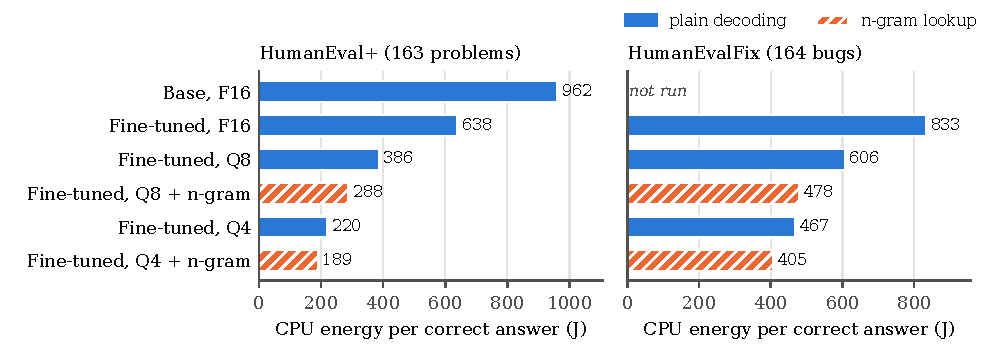
\includegraphics[width=\textwidth]{fig_cpu_energy.pdf}
\caption{Energy per correct answer on the laptop CPU, from the base model in F16 to the fine-tune
in Q4 with n-gram lookup. Base and fine-tuned F16 are from the quantization runs of 14 October,
Q8 and Q4 from the speculative runs of 19 October (Section~\ref{sec:spec}); the base model in F16
was not run on HumanEvalFix.}
\label{fig:cpu}
\end{figure}

Table~\ref{tab:cpu} shows two independent levers, and Figure~\ref{fig:cpu} how they combine with
speculative decoding. \textbf{Quantization} works as expected for a
memory-bound CPU: decode speed follows model size (Q8 1.8$\times$, Q4 2.8$\times$ faster than F16).
Q8 is lossless against F16 (2 of 163 and 9 of 377 answers change, $p\geq0.5$); Q4 costs the
fine-tune 2--4 points on all three benchmarks, none significant alone.

\textbf{Fine-tuning} saves energy without making the model faster: the fine-tune writes about a
third fewer tokens (145 vs.\ 227 on HumanEval+, 50 vs.\ 102 on MBPP+), because its training targets
are bare code, while the base model explains its answer. At equal precision this is 34\% less
energy per solved HumanEval+ problem and 52\% less per solved MBPP+ problem, at accuracy that is
equal (HumanEval+, $p=1$) or higher (MBPP+, +4.0 points, $p=0.077$). On repair the fine-tune solves more
problems with shorter answers: at Q4 it needs 471\,J per fixed bug against 756\,J for the base
model, and fixes 8 points more ($p=0.024$).

\section{Speculative decoding}
\label{sec:spec}

\begin{table}[t]
\centering
\small
\begin{tabular}{llrrrr}
\toprule
 & & \multicolumn{2}{c}{HumanEval+} & \multicolumn{2}{c}{HumanEvalFix} \\
\cmidrule(lr){3-4}\cmidrule(lr){5-6}
Device & Setting & Speed-up & J/correct & Speed-up & J/correct \\
\midrule
CPU, FT Q8 & none & 1.00 & 386 & 1.00 & 606 \\
 & draft Q4, 4 tokens & 1.17 & 367 ($-5\%$) & 1.10 & 665 ($+10\%$) \\
 & draft Q4, 8 tokens & 1.19 & 362 ($-6\%$) & 1.09 & 663 ($+9\%$) \\
 & draft Q8, 8 tokens & 1.10 & 378 ($-2\%$) & 1.03 & 658 ($+9\%$) \\
 & n-gram & \textbf{1.48} & \textbf{288 ($-25\%$)} & \textbf{1.57} & \textbf{478 ($-21\%$)} \\
\midrule
CPU, FT Q4 & none & 1.00 & 220 & 1.00 & 467 \\
 & n-gram & \textbf{1.20} & \textbf{189 ($-14\%$)} & \textbf{1.34} & \textbf{405 ($-13\%$)} \\
\midrule
T4, FT FP16 & none & 1.00 & 325 & 1.00 & 332 \\
 & draft, 2 tokens & 1.88 & 172 ($-47\%$) & 1.47 & 223 ($-33\%$) \\
 & draft, 4 tokens & 1.44 & 210 ($-35\%$) & 1.37 & 240 ($-28\%$) \\
 & draft, 8 tokens & 1.33 & 240 ($-26\%$) & 0.96 & 334 ($+1\%$) \\
 & n-gram, 4 tokens & \textbf{1.96} & \textbf{162 ($-50\%$)} & \textbf{2.44} & \textbf{133 ($-60\%$)} \\
\bottomrule
\end{tabular}
\caption{Speculative decoding for the fine-tune, one request at a time. CPU speed-up is decode
tokens per second relative to plain decoding; T4 speed-up is wall time of plain decoding over
wall time of the setting. The draft is Qwen2.5-Coder-0.5B-Instruct (Q4\_K\_M on the CPU, FP16 on
the T4). N-gram lookup proposes continuations found in the prompt and the text so far.}
\label{tab:spec}
\end{table}

Table~\ref{tab:spec} compares a 0.5B draft model with n-gram lookup. On the \textbf{CPU} the draft
model is accepted 79--91\% of the time, yet speeds decoding up by at most 1.19$\times$ and saves at
most 6\% energy; on repair it costs 9--10\% more than plain decoding. The draft runs on the same four
cores as the target, scoring a block of drafted tokens is not free on a CPU, and the draft also
has to read the prompt, which raises time to first token on repair from 5.7\,s to 7.9\,s. N-gram
lookup proposes tokens at almost no cost, so it wins with lower acceptance (76\% and 58\%): 1.5$\times$
faster, 21--25\% less energy, and no extra memory (1.89\,GB peak vs.\ 2.48--2.66\,GB with a draft).
A Q8 draft was slower than a Q4 draft at equal length, in line with draft latency dominating.
With a Q4 target, n-gram lookup saves about half as much (13--14\%), since a cheaper target leaves
less to save per token; Q4 with n-gram lookup is the cheapest configuration we measured, at 189\,J
per solved HumanEval+ problem and 405\,J per fixed bug.

On the \textbf{T4} verification of a block costs little more than one token, so both methods
help; short drafts work best (2 tokens), and n-gram lookup is again the best setting, halving energy
per correct answer on HumanEval+ and cutting it by 60\% on repair, where the answer mostly copies the
buggy code in the prompt.

\paragraph{Correctness.} Greedy speculative decoding should reproduce plain decoding. Pass counts
indeed move by at most two problems in every setting ($p\geq0.5$), but answers are not bit-identical:
on the CPU 14 of 163 HumanEval+ answers differ with the draft model and 8 with n-gram lookup; on the
T4 155--164 of 163/164 match. Scoring several tokens in one batch changes floating-point rounding;
on the T4 plain decoding at 1 and 8 concurrent requests differs on as many answers.

\section{Fine-tuning shifts the target away from its draft}
\label{sec:shift}

\begin{table}[t]
\centering
\small
\begin{tabular}{lrrrrrr}
\toprule
 & \multicolumn{3}{c}{HumanEval+} & \multicolumn{3}{c}{HumanEvalFix} \\
\cmidrule(lr){2-4}\cmidrule(lr){5-7}
Drafted tokens & 2 & 4 & 8 & 2 & 4 & 8 \\
\midrule
Acceptance, base target & 0.95 & 0.91 & 0.84 & 0.96 & 0.93 & 0.87 \\
Acceptance, fine-tuned target & 0.94 & 0.89 & 0.79 & 0.87 & 0.79 & 0.63 \\
\midrule
Speed-up, base target & 1.60 & 1.42 & 1.24 & 1.40 & 1.43 & 1.47 \\
Speed-up, fine-tuned target & 1.88 & 1.44 & 1.33 & 1.47 & 1.37 & 0.96 \\
\bottomrule
\end{tabular}
\caption{Draft acceptance on the T4, one request at a time, for the same stock 0.5B draft.}
\label{tab:shift}
\end{table}

\begin{figure}[t]
\centering
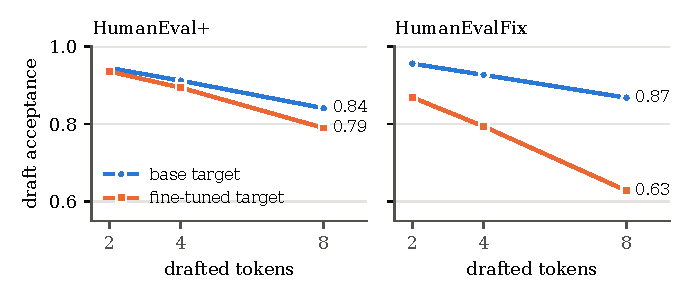
\includegraphics[width=0.7\textwidth]{fig_acceptance.pdf}
\caption{Acceptance of the same stock 0.5B draft for the base and the fine-tuned 1.5B target on
the T4, one request at a time.}
\label{fig:shift}
\end{figure}

The draft model is the base 0.5B model, so it imitates the base 1.5B model better than the
fine-tune. Figure~\ref{fig:shift} and Table~\ref{tab:shift} show the cost. Acceptance is lower for the fine-tuned target at
every length on both benchmarks, and the gap widens with length and on the task the fine-tune was
trained for: on repair it is 0.09 at 2 tokens and 0.24 at 8. With 8 drafted tokens the fine-tune
repairs bugs 4\% more slowly than without speculation, while the base model still gains 1.47$\times$.
For a fine-tuned deployment, a stock draft model should be
used with short drafts, or be fine-tuned or distilled together with the target; n-gram lookup has
no such mismatch.

\section{Batching}
\label{sec:batch}

On the T4, 8 concurrent requests instead of 1 lower energy per correct answer from 325\,J to
36\,J on HumanEval+ for the fine-tune (9$\times$), and from 1007\,J to 142\,J on repair for the base
model (7$\times$); accuracy is unchanged. This is larger than any speculative setting, and it
shrinks speculation's gain: at 8 requests the best draft setting saves at most 19\% and some
lose energy, while n-gram lookup still saves 14--46\%. A local assistant serves one user, so
batching is rarely available on a laptop; speculation is the lever that remains. On the same T4,
CUDA graphs made a single request 1.6$\times$ faster than eager mode, and prefix caching had no
measurable effect on repair prompts that share only a short instruction.

\section{Do the fine-tuning gains replicate?}
\label{sec:seed}

We repeated the fine-tune with a second seed (1234 instead of 3407) and the same data, recipe and
library versions. Against the base model, both seeds gain on MBPP+ (234 vs.\ 212 solved for both
seeds, $p=0.005$) and on HumanEvalFix (59 and 58 vs.\ 41, $p=0.006$ and $0.008$), and neither changes
HumanEval+, CRUXEval-O or completion significantly. One result did not replicate: bug
detection in HumanEvalPack's yes/no format, where the second seed labels almost every function as
buggy (recall 0.95, precision 0.53; accuracy 54.6\% vs.\ 65.6\%), although both seeds score 66\% in
the format they were trained on. We therefore report the generation and repair gains and not the
detection gain.

\section{Related work}

Speculative decoding~\citep{leviathan2023fast,chen2023accelerating} drafts tokens with a cheap
model and verifies them with the target in one pass; \citet{yan2025decoding} show that the speed-up
depends mainly on the draft's latency rather than its accuracy, which our CPU results illustrate
at the extreme where the draft shares the target's compute. Prompt lookup decoding~\citep{saxena2023pld}
replaces the draft model with n-gram matches from the context and suits tasks that copy their input,
such as repair. Energy measurements of LLM inference have mostly targeted large models on
data-centre GPUs~\citep{samsi2023words,luccioni2024power}; we measure a small model on the
hardware it is meant for, and normalise by correct answers.

\section{Limitations}

One model family and size, two devices, Python only, and one run per configuration except for the
seed check; differences under about 10\% in time or energy should not be read as findings.
RAPL covers the CPU package and not memory or the rest of the laptop; T4 board energy includes idle
draw and so favours whatever finishes sooner. The CPU numbers come from unattended sessions on
14 and 19 October; plain decoding measured on both gave 250 and 244\,J per HumanEval+ problem for
Q8 and 141 and 131\,J for Q4, so cross-session comparisons carry a few percent of drift, and the
speculative comparisons are all within one session. Kaggle GPUs are shared.

\section*{Reproducibility and use of AI tools}

Code, prompts, every model answer, logs and power traces are at
\url{https://github.com/MedGm/Locali}; the merged model and the training data are on Hugging Face.
The author used an AI coding assistant (Claude Code) to write much of the evaluation code and
experiment scripts and to draft this text, under the author's direction and review; the research
questions, design and conclusions are the author's, and every number comes from a committed run.

\bibliographystyle{plainnat}
\bibliography{refs}

\end{document}
